Antes de explicar el diseño concreto de cada problema y cómo se implementa en cada tecnología cuántica, en la \textit{fig.~\ref{fig:3-esquema_disenyo}} se indica el flujo de trabajo realizado en este TFG, marcado en color verde se muestran las aportaciones de este trabajo, mientras que en azul se muestran recursos obtenidos de otras fuentes.

\begin{figure}[Flujo de trabajo]{fig:3-esquema_disenyo}{Flujo de trabajo}
  \centering
  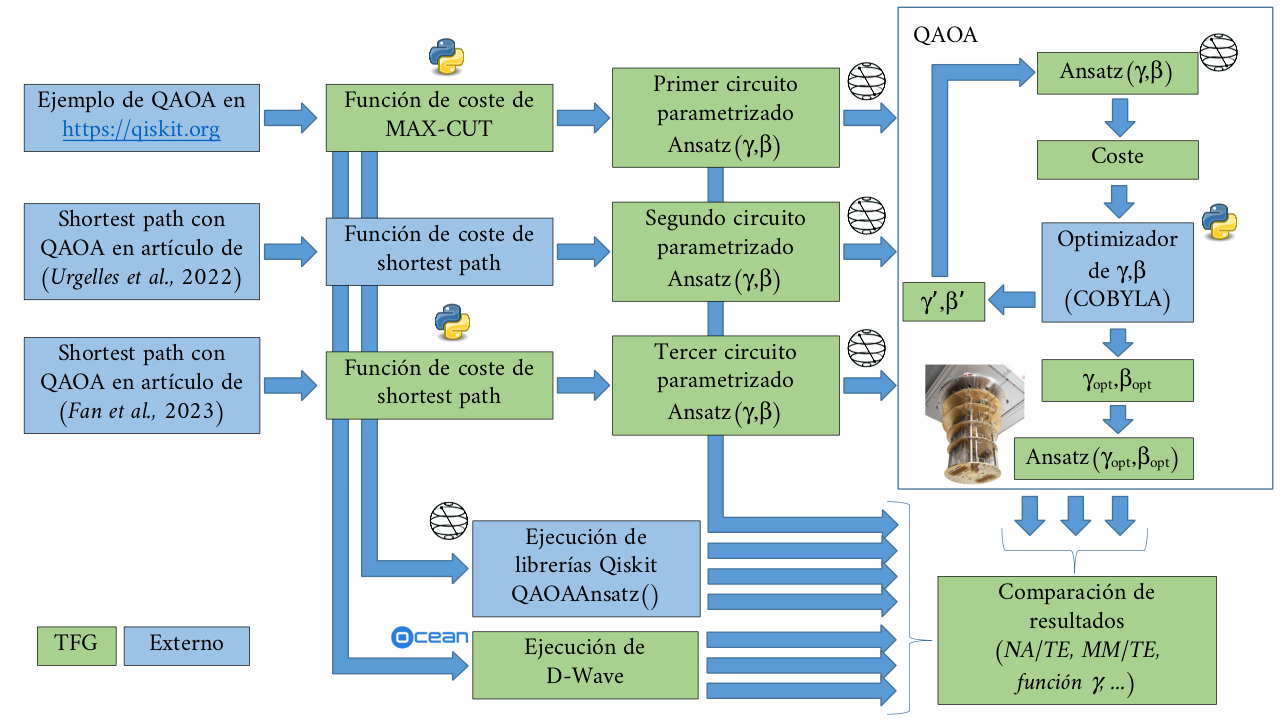
\includegraphics[scale=0.45]{esquema.png}
\end{figure}

Los dos algoritmos del trabajo, QAOA y QA, han sido ejecutados en tres problemas distintos:

\begin{itemize}
\item Max-cut en grafo de 4 aristas:

  Este problema, obtenido en la página web tutorial de Qiskit\cite{qiskit_tutorial_antiguo}, ha sido elegido como el primero a resolver para asegurar una correcta implementación de QAOA, debido a su simplicidad.
  Además, en la fuente se aporta el código utilizado, por lo que se puede comparar completamente con el código propio.
  Los problemas max-cut son un estándar en la resolución de QAOA.

\item Camino más corto en grafo de 4 nodos:

  Tras lograr unos resultados satisfactorios en el problema anterior, se resuelve el problema del artículo de Urgelles et al. (2022)\cite{multi-objective_routing_optimization}.
  En este caso se aumenta la complejidad con respecto a la resolución del problema de max-cut.
  Para comparar con los resultados obtenidos, en el artículo se incluyen un circuito de prueba y estadísticas de QAOA ejecutadas para una y varias capas.

\item Camino más corto para estudiar la variación con el número de capas:

  Tras obtener unos resultados incongruentes en el problema anterior al aumentar el número de capas del algoritmo se decide evaluar otra instancia del problema del camino más corto, del artículo de Fan et al. (2023)\cite{solving_shortest_path_with_qaoa}, para analizar el comportamiento del algoritmo para $p > 1$.
\end{itemize}

Para estos tres casos se ha seguido el mismo proceso de análisis.
\\
Se ha definido una función de coste clásica apta para el problema.
Después se ha utilizado esta función para calcular el circuito parametrizado ansatz.
Este se ha aplicado en una implementación realizada en Python del algoritmo haciendo uso de la librería de Qiskit, que permite la construcción y posterior ejecución de circuitos cuánticos a nivel de puertas.
\\
Por otra parte la función de coste también ha sido utilizada para la ejecución de QA en ordenadores de D-Wave y para la ejecución de la función \textit{Qiskit.QAOAAnsatz()}, la cual es una implementación de caja negra de QAOA empleada para su comparación con el código escrito.
\\
El análisis de los resultados ha sido realizado utilizando como datos los proporcionados por las respectivas fuentes de los problemas, además de los resultados de las ejecuciones de QA, QAOA y \textit{Qiskit.QAOAAnsatz()}, así como los circuitos generados por las dos últimas.
Las métricas empleadas para esta comparación han sido definidas en el capítulo~\ref{CAP:RESULTADOS}.

Para llevar este proceso a cabo es necesario comprender antes cómo funciona QAOA y cómo se puede formular un problema de optimización con restricciones para que sea resuelto por este algoritmo.

\section{Traducción de problemas de optimización combinatoria a QUBO\label{sec:3-problemas de optimizacion combinatoria}}{disenyo/qbo_a_qubo.tex}

\section{Circuito de QAOA\label{sec:3-circuito de qaoa}}{disenyo/circuito_qaoa.tex}

\section{Algoritmo de QAOA}{disenyo/algoritmo_qaoa.tex}


%%% Local Variables:
%%% mode: latex
%%% TeX-master: "../tfgtfmthesisuam"
%%% End:
